\documentclass{article}
\usepackage{amsmath}
\usepackage{amssymb}
\usepackage{ctex}
\usepackage[margin=2cm]{geometry} % 设置较窄的边距使文档宽一些
\usepackage{multirow} % 支持表格中的多行单元格
\usepackage{graphicx} % 用于插入图片
\usepackage{subcaption} % 支持子标题
\usepackage{float} % 支持 [H] 浮动体选项
\title{\heiti\zihao{2}实验名称 }
\author{\songti  姓名  学号 \\
课程号  XXXX.01 }
\date{2025.5.20}
\begin{document}
    \maketitle
\begin{abstract}
    \noindent{\textbf{摘要:} }
    
    \noindent{\textbf{关键词:} }
\end{abstract}
\section{实验目的}
\begin{enumerate}
    \item 
\end{enumerate}

\section{实验原理}

\section{实验器材}
\label{sec:equipment}
    \begin{enumerate}
        \item 
    \end{enumerate} 

\section{实验内容}
\subsection{ }

\begin{figure}[H]
    \centering
    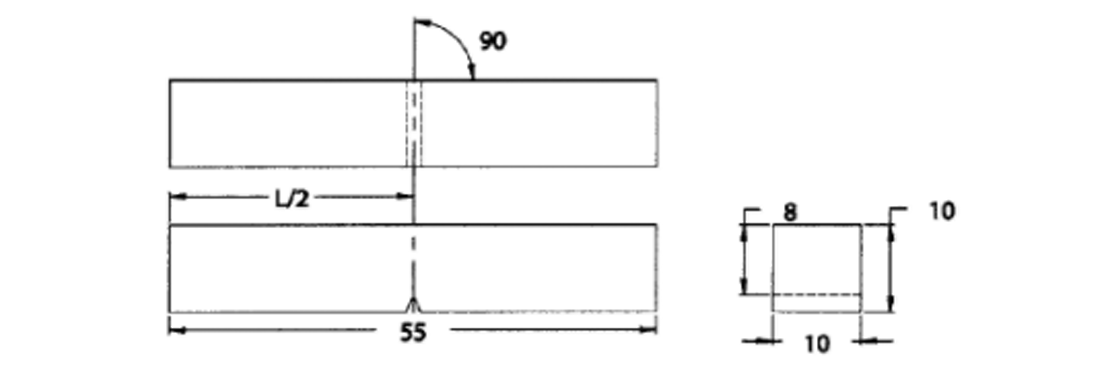
\includegraphics[width=0.8\textwidth]{img1.png}
    \caption{图片描述}
    \label{fig:star_connection_circuit}
\end{figure}





\section{预习思考题 }
\subsection{ }
\subsection{ }


\subsection{ }




\section{总结感悟 }

\section{参考文献}
\begin{enumerate}
    \item 
\end{enumerate} 

\end{document}

\end{document}